\begin{definicion}{Concepto de función (1 día)}
\end{definicion}    
\begin{definicion}{Dominio de una función}
\end{definicion}
\begin{ejercicios}
\ej Encuentra el dominio de las siguientes funciones:
\begin{apartadosc}
 \ap $f(x)=\dfrac{x+1}{2x^2+x}$
    \sol{$\dom(f)=\mathbb{R}-\{-\frac12,0\}$}
 \ap $f(x)=\sqrt{6-x-x^2}$
    \sol{$\dom(f)=[-3,2]$}
 \ap $f(x)=\ln{(3x+2)}$
    \sol{$\dom(f)=(-\frac32,\infty)$}
 \ap $\displaystyle{f(x)=\sqrt{2-x}-\sqrt{x}}$
    \sol{$\dom(f)=[0,2]$}
 \ap $\ln\dfrac{x+2}{x-1}$
    \sol{$\dom(f)=(-\infty,-2)\cup(1,\infty)$}
 \ap $f(x)=\dfrac{x+2}{\ln{x}}$
    \sol{$\dom(f)=(0,1)\cup(1,\infty)$}
\end{apartadosc}
\end{ejercicios}

\Punto{Límite de una función en un punto}
\begin{definicion}{Límite de una función en un punto (2 días)}
Decimos que una función $f(x)$ tiene límite $L$ cuando $x$ tiende a $x_0$ si podemos aproximar tanto como queramos $f(x)$ a $L$, tomando valores de $x$ suficientemente próximos a $x_0$.
$$
    \lim_{x\,\to\,x_0}f(x)=L
        \quad\Longleftrightarrow\quad
    \forall\varepsilon>0,\,\exists\,\delta>0\,\mid\,|f(x)-L|<\varepsilon\text{ si }0<|x-x_0|<\delta
$$
\centerline{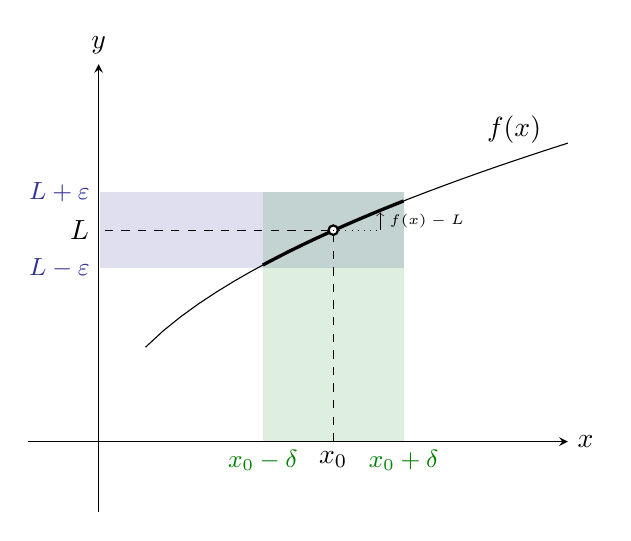
\begin{tikzpicture}
    \begin{axis}[
        axis lines=middle,
        xlabel={$x$},
        ylabel={$y$},
        xmin=-1.5, xmax=10,
        ymin=-0.75, ymax=4,
        every axis x label/.style={at={(current axis.right of origin)}, anchor=west},
        every axis y label/.style={at={(current axis.above origin)}, anchor=south},
        ticks=none,
        axis line style={-stealth},
    ]
        \fill[blue!50!black,opacity=0.125]
            (0.02,1.84) node[left,opacity=0.8] {\small $L-\varepsilon$} -- 
            (0.02,2.64) node[left,opacity=0.8] {\small $L+\varepsilon$} -- 
            (6.5,2.64) -- 
            (6.5,1.84) -- 
            cycle;
        \fill[green!50!black,opacity=0.125]
            (3.5,0.01) node[below,opacity=1] {\small $x_0-\delta$} --
            (3.5,2.64) --
            (6.5,2.64) --
            (6.5,0.01) node[below,opacity=1] {\small $x_0+\delta$} --
            cycle;
        \addplot[domain=1:10]{x^0.5} node[above=1mm,very near end] {$f(x)$};
        \addplot[very thick,domain=3.5:6.5]{x^0.5};
        \draw[thin,dashed]  (5,0) node[below] {$x_0$} --
                    (5,2.24) --
                    (0,2.24) node[left] {$L$};
        \filldraw[thick,fill=white] (5,2.24) ellipse (0.1 and 0.05);
        \draw[very thin,->] (6,2.24) -- (6,2.43) node[right,midway] {\tiny $f(x)-L$};
        \draw[very thin,dotted] (5,2.24) -- (6,2.24);
    \end{axis}
\end{tikzpicture}}
Intuitivamente, el límite de una función en un punto nos dice el valor al que se acerca la función cuando $x$ se acerca todo lo que queramos a $x_0$, sin llegar a dicho punto. Así, una expresión como esta:
$$\lim_{x\,\to\,5}f(x)=3$$
debe interpretarse como: \emph{Si tomamos valores de $x$ infinitamente cercanos a $5$, la función tomará valores infinitamente cercanos a $3$}.

\vspace{3mm}\centerline{
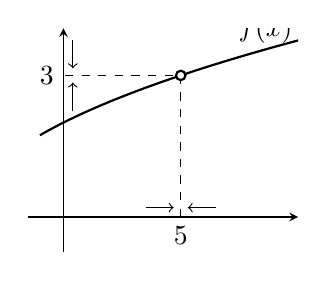
\begin{tikzpicture}
    \begin{axis}[
        scale=0.5,
        axis lines=middle,
        xmin=-1.5, xmax=10,
        ymin=-0.75, ymax=4,
        ticks=none,
        axis line style={-stealth},
    ]
        \addplot[thick,domain=-1:10,samples=500]{(x+4)^0.5}
            node[above=-0.5mm,very near end] {$f(x)$};
        \draw[thin,dashed]  (5,0)  node[below] {$5$} -- 
                            (5,3) -- 
                            (0,3) node[left] {$3$};
        \filldraw[thick,fill=white] (5,3) ellipse (0.2 and 0.1);
        \draw[->] (3.5,0.2) -- (4.7,0.2);
        \draw[->] (6.5,0.2) -- (5.3,0.2);
        \draw[->] (0.4,2.25) -- (0.4,2.85);
        \draw[->] (0.4,3.75) -- (0.4,3.15);
    \end{axis}
\end{tikzpicture}}

Si esto no es posible decimos que la función no tiene límite en el punto. Las siguientes gráficas son ejemplos de funciones sin límite en $x_0$:

\vspace{3mm}\centerline{
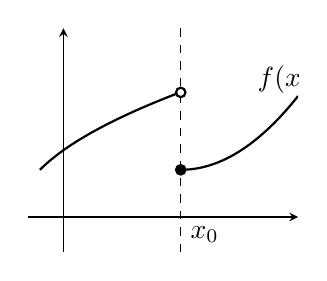
\begin{tikzpicture}
    \begin{axis}[
        scale=0.5,
        axis lines=middle,
        xmin=-1.5, xmax=10,
        ymin=-0.75, ymax=4,
        ticks=none,
        axis line style={-stealth},
    ]
        \addplot[thick,domain=-1:4.99,samples=500]{(x+2)^0.5};
        \addplot[thick,domain=5.01:10,samples=500]{1+(0.25*x-1.25)^2} node[above=1mm,very near end] {$f(x)$};
        \draw[thin,dashed] (5,-0.75) -- (5,0) node[below right] {$x_0$} -- (5,4);
        \filldraw[thick,fill=white] (5,2.64) ellipse (0.2 and 0.1);
        \filldraw[thick,fill=black] (5,1) ellipse (0.2 and 0.1);
    \end{axis}
\end{tikzpicture}\hspace{10mm}
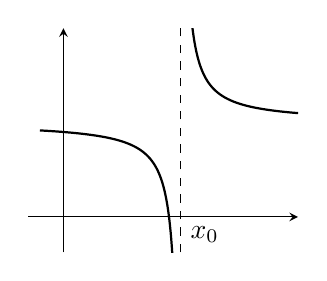
\begin{tikzpicture}
    \begin{axis}[
        scale=0.5,
        axis lines=middle,
        xmin=-1.5, xmax=10,
        ymin=-0.75, ymax=4,
        ticks=none,
        axis line style={-stealth},
    ]
        \addplot[thick,domain=-1:4.99,samples=500]{2+(1/(x-5))};
        \addplot[thick,domain=5.01:10,samples=500]{2+(1/(x-5))} node[above=1mm,very near end] {$f(x)$};
        \draw[thin,dashed] (5,-0.75) -- (5,0) node[below right] {$x_0$} -- (5,4);
    \end{axis}
\end{tikzpicture}}
\end{definicion}

\begin{definicion}{Propiedades de los límites}
Sean $f(x)$ y $g(x)$ dos funciones con límites finitos en $x_0$ y sea $k\in\mathbb{R}$ una constante. Entonces se cumplen las siguientes propiedades, con las condiciones indicadas:
\begin{itemize}
    \item[\pr{L1.}] $\displaystyle\lim_{x\to x_0}k=k$.
    \item[\pr{L2.}] $\displaystyle\lim_{x\to x_0}x=x_0$.
    \item[\pr{L3.}] $\displaystyle\lim_{x\to x_0}(f\pm g)(x)=\lim_{x\to x_0}f(x)\pm\lim_{x\to x_0}g(x)$.
    \item[\pr{L4.}] $\displaystyle\lim_{x\to x_0}(f\cdot g)(x)=\lim_{x\to x_0}f(x)\cdot\lim_{x\to x_0}g(x)$.
    \item[\pr{L5.}] $\displaystyle\lim_{x\to x_0}\left(\frac fg\right)(x)=\frac{\displaystyle\lim_{x\to x_0}f(x)}{\displaystyle\lim_{x\to x_0}g(x)}$, si $\displaystyle\lim_{x\to x_0}g(x)\ne0$.
    \item[\pr{L6.}] $\displaystyle\lim_{x\to x_0}\left[f(x)^{g(x)}\right]=\left[\lim_{x\to x_0}f(x)\right]^{\displaystyle\lim_{x\to x_0}g(x)}$, si $\displaystyle\lim_{x\to x_0}f(x)>0$.
    \item[\pr{L7.}] $\displaystyle\lim_{x\to x_0}f\bigl(g(x)\bigr)=f\left(\lim_{x\to x_0}g(x)\right)$, si $f$ es continua en $\displaystyle\lim_{x\to x_0}g(x)$.
\end{itemize}
Demostrarlas requiere manipular directamente la definición anterior, y el proceso necesita herramientas que exceden el nivel de este curso.
\end{definicion}

\begin{definicion}{Límites determinados}
Las propiedades de los límites permiten calcular muchos límites simplemente sustituyendo la variable $x$ por el valor al que tiende. Cuando esto es posible decimos que el límite es \emph{determinado}.
\end{definicion}

\begin{ejemplo}{
Calcula el valor de los siguientes límites. En el segundo, estudia los límites laterales e indica si existe el límite bilateral:
\begin{apartadosc}
 \ap $\displaystyle{\lim_{x\,\to\,3}\dfrac{x^2+x}{x-1}}$
 \ap $\displaystyle{\lim_{x\,\to\,-2}\dfrac{x+3}{x+2}}$
 \ap $\displaystyle{\lim_{x\,\to\,0}\dfrac{e^x-1}{x^2+1}}$
 \ap $\displaystyle{\lim_{x\,\to\,e}\dfrac{\ln{x}}{1+\ln{x^2}}}$
\end{apartadosc}
}
\end{ejemplo}

\begin{definicion}{Límites laterales}
Hasta ahora hemos hablado de que la variable $x$ se acerca a un valor $x_0$, pero hemos obviado que esta aproximación se puede hacer desde dos direcciones distintas: por la izquierda, tomando valores de $x$ menores que $x_0$; o por la derecha, tomando valores de $x$ mayores que $x_0$.

\vspace{3mm}\centerline{
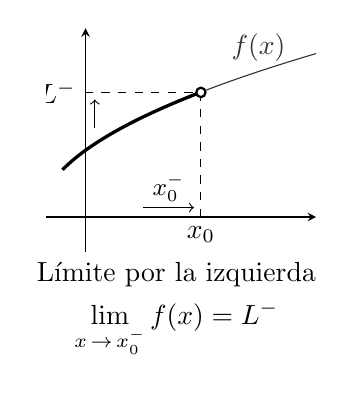
\begin{tikzpicture}
    \begin{axis}[
        scale=0.5,
        axis lines=middle,
        xmin=-1.7, xmax=10,
        ymin=-0.75, ymax=4,
        ticks=none,
        axis line style={-stealth},
    ]
        \addplot[very thick,domain=-1:5,samples=500]{(x+2)^0.5};
        \addplot[thin,black!80,domain=5:10,samples=500]{(x+2)^0.5}
            node[above,midway] {$f(x)$};
        \draw[thin,dashed]  (5,0)  node[below] {$x_0$} -- 
                            (5,2.64) -- 
                            (0,2.64) node[left] {$L^-$};
        \filldraw[thick,fill=white] (5,2.64) ellipse (0.2 and 0.1);
        \draw[->] (2.5,0.2) -- (4.7,0.2) node[above=-0.5mm,midway] {\small $x^-_0$};
        \draw[->] (0.4,1.89) -- (0.4,2.49);
    \end{axis}
    \node[below] at (1.65,0) {Límite por la izquierda};
    \node[below] at (1.65,-0.5) {$\displaystyle{\lim_{x\,\to\,x_0^-}f(x)=L^-}$};
\end{tikzpicture}\hspace{1cm}
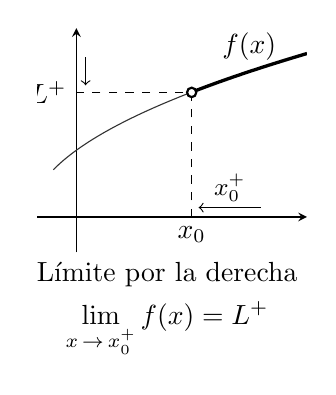
\begin{tikzpicture}
    \begin{axis}[
        scale=0.5,
        axis lines=middle,
        xmin=-1.7, xmax=10,
        ymin=-0.75, ymax=4,
        ticks=none,
        axis line style={-stealth},
    ]
        \addplot[thin,black!80,domain=-1:5,samples=500]{(x+2)^0.5};
        \addplot[very thick,domain=5:10,samples=500]{(x+2)^0.5}
            node[above,midway] {$f(x)$};
        \draw[thin,dashed]  (5,0)  node[below] {$x_0$} -- 
                            (5,2.64) -- 
                            (0,2.64) node[left] {$L^+$};
        \filldraw[thick,fill=white] (5,2.64) ellipse (0.2 and 0.1);
        \draw[->] (8,0.2) -- (5.3,0.2) node[above=-0.5mm,midway] {\small $x^+_0$};;
        \draw[->] (0.4,3.39) -- (0.4,2.79);
    \end{axis}
    \node[below] at (1.65,0) {Límite por la derecha};
    \node[below] at (1.65,-0.5) {$\displaystyle{\lim_{x\,\to\,x_0^+}f(x)=L^+}$};
\end{tikzpicture}}

Los límites laterales se calculan como cualquier otro límite, pero teniendo en cuenta que las expresiones que tienden a $0$ tienen un signo definido que hay que razonar para hacer los cálculos.
\end{definicion}

\begin{ejemplo}{
Calcula el valor de los siguientes límites:
\begin{apartadosc}
 \ap $\displaystyle{\lim_{x\,\to\,1^+}\dfrac{3x+2}{x^2-1}=\dfrac5{0^+}=+\infty}$
 \ap $\displaystyle{\lim_{x\,\to\,\pi^-}\dfrac{1-\cos{x}}{\sen{x}}=\dfrac2{+0}=+\infty}$
 \ap $\displaystyle{\lim_{x\,\to\,1^-}\dfrac{x+1}{\ln{x}}=\dfrac2{-0}=-\infty}$
 \ap $\displaystyle{\lim_{x\,\to\,0^+}\dfrac{x+1}{\ln{x}}=0}$
\end{apartadosc}
}
\end{ejemplo}

\begin{definicion}{Indeterminación $\left[\frac00\right]$}
Es frecuente que al calcular límites aplicando las propiedades obtengamos el resultado indecidible $0/0$, tendremos entonces que volver a la expresión original, reescribirla y simplificarla, hasta que la indeterminación desaparezca. La forma en que conseguimos nuestro propósito dependerá de la naturaleza de la expresión, como se muestra en el siguiente ejemplo.
\end{definicion}

\begin{ejemplo}{
Calcula el valor de los siguientes límites:
\begin{apartadosc}
 \ap $\displaystyle{\lim_{x\,\to\,2}\dfrac{x^2-4}{2x-4}}$
 \ap $\displaystyle{\lim_{x\,\to\,-1^-}\dfrac{1-x^2}{(x+1)^2}}$
 \ap $\displaystyle{\lim_{x\,\to\,1^+}\dfrac{\sqrt{x}-1}{x-1}}$
 \ap $\displaystyle{\lim_{x\,\to\,1^+}\dfrac{\sqrt{x-1}}{\sqrt{x}-1}}$
\end{apartadosc}
}
\metodo{Apartado a}

Para funciones racionales bastará con factorizar los polinomios implicados y simplificar los factores comunes.
\[\begin{aligned}
    \lim_{x\,\to\,2}\dfrac{x^2-4}{2x-4}&=\left[\dfrac00\right]\\
        &=\lim_{x\,\to\,2}\dfrac{(x+2)\cdot(x-2)}{2(x-2)}=\\
        &=\lim_{x\,\to\,2}\dfrac{x+2}{2}=2
\end{aligned}\]
\metodo{Apartado b}

\[\begin{aligned}
    \lim_{x\,\to\,-1^-}\dfrac{1-x^2}{(x+1)^2}&=\left[\dfrac00\right]\\
        &=\lim_{x\,\to\,-1^-}\dfrac{(1-x)\cdot(1+x)}{(x+1)^2}=\\
        &=\lim_{x\,\to\,-1^-}\dfrac{1-x}{x+1}=-\infty
\end{aligned}\]
\metodo{Apartado c}

Si aparecen raíces en el numerador o en el denominador deberemos multiplicar y dividir por el conjugado para revelar los factores implicados.
\[\begin{aligned}
    \lim_{x\,\to\,1^+}\dfrac{\sqrt{x}-1}{x-1}&=\left[\dfrac00\right]\\
        &=\lim_{x\,\to\,1^+}\dfrac{\sqrt{x}-1}{x-1}\cdot\dfrac{\sqrt{x}+1}{\sqrt{x}+1}=\\
        &=\lim_{x\,\to\,1^+}\dfrac{\left(\sqrt{x}\right)^2-1^2}{(x-1)\cdot\left(\sqrt{x}+1\right)}=\\
        &=\lim_{x\,\to\,1^+}\dfrac{x-1}{(x-1)\cdot\left(\sqrt{x}+1\right)}=\\
        &=\lim_{x\,\to\,1^+}\dfrac{1}{\sqrt{x}+1}=\dfrac12
\end{aligned}\]
\metodo{Apartado d}

\[\begin{aligned}
    \lim_{x\,\to\,1^+}\dfrac{\sqrt{x-1}}{\sqrt{x}-1}&=\left[\dfrac00\right]\\
        &=\lim_{x\,\to\,1^+}\dfrac{\sqrt{x-1}}{\sqrt{x}-1}
            \cdot\dfrac{\sqrt{x-1}}{\sqrt{x-1}}
                \cdot\dfrac{\sqrt{x}+1}{\sqrt{x}+1}=\\
        &=\lim_{x\,\to\,1^+}\dfrac{\left(\sqrt{x-1}\,\right)^2}{\left[\left(\sqrt{x}\right)^2-1^2
        \right]\cdot\sqrt{x-1}}=\\
        &=\lim_{x\,\to\,1^+}\dfrac{x-1}{(x-1)\cdot\sqrt{x-1}}=\\
        &=\lim_{x\,\to\,1^+}\dfrac{1}{\sqrt{x-1}}=+\infty
\end{aligned}\]
\end{ejemplo}

\begin{ejercicios}
 \ej Ejercicios 1 y 5 del repertorio
\end{ejercicios}

\Punto{Pendiente y derivada}
\begin{definicion}{1 día}
\end{definicion}

\begin{ejemplo}
{
    Calcula las siguientes derivadas aplicando la definición:
    \begin{apartados}
     \ap $f(x)=3x^2-2$
     \ap $g(x)=\sqrt{3x+1}$
    \end{apartados}
}
\metodo{Apartado a}
\[\begin{aligned}
    f'(x)&=\lim_{h\,\to\,0}\dfrac{3(x+h)^2-2-(3x^2-2)}{h}=\left[\dfrac00\right]\\
        &=\lim_{h\,\to\,0}\dfrac{3x^2+6hx+3h^2-2-3x^2+2}{h}=\\
        &=\lim_{h\,\to\,0}\dfrac{6hx+3h^2}{h}=\\
        &=\lim_{h\,\to\,0}\dfrac{h\cdot(6x+3h)}{h}=\\
        &=\lim_{h\,\to\,0}(6x+3h)=6x\\
\end{aligned}\]

\metodo{Apartado b}
\[\begin{aligned}
    g'(x)&=\lim_{h\,\to\,0}\dfrac{\sqrt{3(x+h)+1}-\sqrt{3x+1}}{h}=\left[\dfrac00\right]\\
        &=\lim_{h\,\to\,0}\dfrac{\sqrt{3x+3h+1}-\sqrt{3x+1}}{h}
            \cdot\dfrac{\sqrt{3x+3h+1}+\sqrt{3x+1}}{\sqrt{3x+3h+1}+\sqrt{3x+1}}=\\
        &=\lim_{h\,\to\,0}\dfrac{3x+3h+1-(3x+1)}{h\cdot\left(\sqrt{3x+3h+1}+\sqrt{3x+1}\right)}=\\
        &=\lim_{h\,\to\,0}\dfrac{3h}{h\cdot\left(\sqrt{3x+3h+1}+\sqrt{3x+1}\right)}=\\
        &=\lim_{h\,\to\,0}\dfrac{3}{\sqrt{3x+3h+1}+\sqrt{3x+1}}=\dfrac{3}{2\sqrt{3x+1}}
\end{aligned}\]
\end{ejemplo}

\Punto{Obtención de la derivada}

\begin{definicion}{Fórmulas y Propiedades}
\end{definicion}

\begin{ejemplo}{
Calcula la derivada de las siguientes funciones:
\begin{apartados}
    \ap $y=5\pi$
    \ap $y=3x-2$
    \ap $y=\dfrac{2-x}3$
    \ap $y=x^7$
    \ap $y=\sqrt[3]{x}$
    \ap $y=\dfrac1{x^4}$
    \ap $y=5\sqrt{x^3}$
    \ap $y=3\ln{x}-2\cos{x}+2$
    \ap $y=x^2\ln{x}$
    \ap $y=\dfrac{2x+1}{x+1}$
    \ap $y=\dfrac{\sqrt{x}}{x-1}$
    \ap $y=\dfrac{\sen{x}}{1+\sen{x}}$
\end{apartados}
}
\metodo{Apartado a:}\quad $y=5\pi$

\vspace{2mm}Se trata de una función constante, y su gráfica es una recta horizontal de pendiente nula, así que su derivada debe ser cero.
\[y'\ueq{F1}0\]

\metodo{Apartado b:}\quad $y=3x-2$

\vspace{2mm}Se trata de una función lineal, así que su derivada coincide con la pendiente:
\[y'\ueq{F2}3\]

\metodo{Apartado c:}\quad $y=\dfrac{2-x}3$

\vspace{2mm}Si separamos la fracción nos daremos cuenta de que también se trata de una función lineal:
\[y=\dfrac23-\dfrac13\cdot x\]
y entonces su derivada es:
\[y'\ueq{F2}-\dfrac13\]

\metodo{Apartado d:}\quad $y=x^7$
\[y'\ueq{F3}7\cdot x^{7-1}=7x^6\]

\metodo{Apartado e:}\quad $y=\sqrt[3]{x}$

Aunque la tabla tiene fórmulas específicas para derivar raíces de cualquier índice, mi consejo es que utilicéis también F3 para esta derivada, expresándola primero en forma de potencia:
\[y=\sqrt[3]{x}=x^{1/3}\]
Entonces:
\[y'\ueq{F3}\frac13\cdot x^{1/3-1}=\frac13\cdot x^{-2/3}=\frac1{3\sqrt[3]{x^2}}\]

\metodo{Apartado f:}\quad $y=\dfrac1{x^4}$

La misma idea permite derivar fracciones cuyo numerador es constante:
\[y=\frac1{x^4}=x^{-4}\]
Entonces:
\[y'\ueq{F3}-4\cdot x^{-4-1}=-4\cdot x^{-5}=-\frac4{x^5}\]

\metodo{Apartado g:}\quad $y=5\sqrt{x^3}$

A partir de aquí empezamos a necesitar las propiedades de las derivadas.
\[y=5\cdot x^{3/2}\]
 P1 nos dice que \emph{las constantes multiplicativas no se derivan}. Entonces:
\[y'=\left(5\cdot x^{3/2}\right)'\oeq{P1}
    5\cdot\left(x^{3/2}\right)'\ueq{F3}
    5\cdot\frac32\cdot x^{1/2}=\frac{15\sqrt{x}}2
\]

\metodo{Apartado h:}\quad $y=3\ln{x}-2\cos{x}+2$

La propiedad P2 nos dice que en el caso de sumas y restas, cada término se debe derivar por separado

\[\begin{aligned}
    y'&=\left(3\ln{x}-2\cos{x}+2\right)'=\\
        &\oeq{P2}\left(3\ln{x}\right)'-\left(2\cos{x}\right)'+2'=\\
        &\oeq{P1}3\cdot\left(\ln{x}\right)'-2\cdot\left(\cos{x}\right)'+2'=\\
        &\ueq{F6\\F7\\F1}3\cdot\frac1x-2\cdot\left(-\sen{x}\right)+0=\frac3x+2\sen{x}
\end{aligned}\]

\metodo{Apartado i:}\quad $y=x^2\ln{x}$

Para derivar productos utilizamos P3. ¡Cuidado!, esta fórmula no es tan intuitiva como las anteriores, no basta con derivar cada factor por separado.

\[\begin{aligned}
    y'&=\left(x^2\cdot\ln{x}\right)'=\\
        &\oeq{P3}\left(x^2\right)'\cdot\ln{x}+x^2\cdot\left(\ln{x}\right)'=\\
        &\ueq{F3\\F6}2x\cdot\ln{x}+x^2\cdot\frac1x=\\
        &=2x\ln{x}+x=x\cdot(1+2\ln{x})
\end{aligned}\]

\metodo{Apartado j:}\quad $y=\dfrac{2x+1}{x+1}$

Derivamos con P4.

\[\begin{aligned}
    y'&=\left(\frac{2x+1}{x+1}\right)'=\\
        &\oeq{P4}\dfrac{\left(2x+1\right)'\cdot(x+1)-(2x+1)\cdot\left(x+1\right)'}{(x+1)^2}=\\
        &\ueq{F2}\dfrac{2\cdot(x+1)-(2x+1)\cdot1}{(x+1)^2}=\dfrac1{(x+1)^2}
\end{aligned}\]

\metodo{Apartado k:}\quad $y=\dfrac{\sqrt{x}}{x-1}$
\[\begin{aligned}
    y'&=\left(\frac{\sqrt{x}}{x-1}\right)'=\\
        &\oeq{P4}\dfrac{\left(\sqrt{x}\right)'\cdot(x-1)-\sqrt{x}\cdot\left(x-1\right)'}{(x-1)^2}=\\
        &\ueq{F2}\dfrac{\frac1{2\sqrt{x}}\cdot(x-1)-\sqrt{x}\cdot1}{(x-1)^2}=\\
        &\uoeq{\cdot2\sqrt{x}}{\cdot2\sqrt{x}}\dfrac{(x-1)-2x}{2\sqrt{x}\cdot(x-1)^2}
            =-\frac{x+1}{2\sqrt{x}\cdot(x-1)^2}
\end{aligned}\]

\metodo{Apartado l:}\quad $y=\dfrac{\sen{x}}{1+\sen{x}}$
\[\begin{aligned}
    y'&=\left(\frac{\sen{x}}{1+\sen{x}}\right)'=\\
        &\oeq{P4}\dfrac{\left(\sen{x}\right)'\cdot(1+\sen{x})-\sen{x}\cdot\left(1+\sen{x}\right)'}{(1+\sen{x})^2}=\\
        &\ueq{F7}\dfrac{\cos{x}\cdot(1+\sen{x})-\sen{x}\cdot\cos{x}}{(1+\sen{x})^2}=\frac{\cos{x}}{(1+\sen{x})^2}
\end{aligned}\]

\end{ejemplo}

\begin{ejemplo}{
Calcula la derivada de las siguientes funciones aplicando la regla de la cadena:
 \begin{apartadosc}
  \ap $y=(2x-3)^3$
  \ap $y=\sen\sqrt{x}$
  \ap $y=\sqrt{\sen{x}}$
  \ap $y=2\ln{(x^2+x)}$
  \ap $y=\ln{\tan{x}+\tan{\ln{x}}}$
  \ap $y=x\arctan{x^2}$
  \ap $y=\dfrac{x^2+1}{(1-2x)^2}$
  \ap $y=\dfrac{e^{1-x}}{e^{1-x}+1}$
  \ap $y=\arcsen{\dfrac1x}$
 \end{apartadosc}}
 \metodo{Apartado a:}\quad $y=(2x-3)^3$
\[\begin{aligned}
    y'&=\left[(2x-3)^3\right]'=\\
        &\uoeq{F5}{P5}3\cdot(2x-3)^2\cdot(2x-3)'=\\
        &\ueq{F2}3\cdot(2x-3)^2\cdot2=6\cdot(2x-3)^2
\end{aligned}\]

 \metodo{Apartado b:}\quad $y=\sen\sqrt{x}$
\[\begin{aligned}
    y'&=\left(\sen\sqrt{x}\right)'=\\
        &\uoeq{F7}{P5}\left(\sqrt{x}\,\right)'\cos\sqrt{x}=\\
        &\ueq{F3}\frac1{2\sqrt{x}}\cdot\cos\sqrt{x}=\frac{\cos\sqrt{x}}{2\sqrt{x}}
\end{aligned}\]

 \metodo{Apartado c:}\quad $y=\sqrt{\sen{x}}$
\[\begin{aligned}
    y'&=\left(\sqrt{\sen{x}}\right)'=\\
        &\uoeq{F3}{P5}\frac1{2\sqrt{\sen{x}}}\cdot(\sen{x})'=\\
        &\ueq{F7}\frac1{2\sqrt{\sen{x}}}\cdot\cos{x}=\frac{\cos{x}}{2\sqrt{\sen{x}}}
\end{aligned}\]

 \metodo{Apartado d:}\quad $y=2\ln{(x^2+x)}$
\[\begin{aligned}
    y'&=\left[2\ln{(x^2+x)}\right]'=\\
        &\oeq{P1}2\left[\ln{(x^2+x)}\right]'=\\
        &\uoeq{F6}{P5}2\cdot\frac1{x^2+x}\cdot(x^2+x)'=\\
        &=2\cdot\frac1{x^2+x}\cdot(2x+1)=\frac{4x+2}{x^2+x}
\end{aligned}\]

 \metodo{Apartado e:}\quad $y=\ln\left(\tan x+\tan(\ln x)\right)$
\[\begin{aligned}
    y'&=\frac{\left(\tan x+\tan(\ln x)\right)'}{\tan x+\tan(\ln x)}\\
      &=\frac{(\tan x)'+\left(\tan(\ln x)\right)'}{\tan x+\tan(\ln x)}\\
      &=\frac{\dfrac1{\cos^2 x}+\dfrac1{\cos^2(\ln x)}\cdot\dfrac1x}
              {\tan x+\tan(\ln x)}.
\end{aligned}\]

 \metodo{Apartado f:}\quad $y=x\cdot\arctan{x^2}$
\[\begin{aligned}
    y'&=\left(x\cdot\arctan{x^2}\right)'=\\
        &=x'\cdot\arctan{x^2}+x\cdot\left(\arctan{x^2}\right)'=\\
        &=1\cdot\arctan{x^2}+x\cdot\frac1{1+(x^2)^2}\cdot2x=\frac{2x^2}{1+x^4}+\arctan{x^2}
\end{aligned}\]

 \metodo{Apartado g:}\quad $y=\dfrac{x^2+1}{(1-2x)^2}$
 \[\begin{aligned}
    y'&=\dfrac{2x\cdot(1-2x)^2-(x^2+1)\cdot2\cdot(1-2x)\cdot(-2)}{(1-2x)^4}=\\
        &=\dfrac{2x\cdot(1-2x)+4\cdot(x^2+1)}{(1-2x)^3}
            =\dfrac{2x+4}{(1-2x)^3}
\end{aligned}\]

 \metodo{Apartado h:}\quad $y=\dfrac{e^{1-x}}{e^{1-x}+1}$
 \[y'=\dfrac{-e^{1-x}\cdot(e^{1-x}+1)-e^{1-x}\cdot(-e^{1-x})}{(e^{1-x}+1)^2}
        =-\dfrac{e^{1-x}}{(e^{1-x}+1)^2}
\]

 \metodo{Apartado i:}\quad $y=\arcsen\dfrac1{x}$
 \[\begin{aligned}
    y'&=\dfrac1{\sqrt{1-\left(\dfrac1x\right)^2}}\cdot\left(\frac1x\right)'=\\
        &=\dfrac1{\sqrt{1-\dfrac1{x^2}}}\cdot\dfrac{-1}{x^2}
            =-\dfrac{1}{\sqrt{x^4-x^2}}
\end{aligned}\]

\end{ejemplo}

\Punto{Recta tangente}
\begin{definicion}{1 día}
\end{definicion}

\begin{ejemplo}{
    Calcula la ecuación de la recta tangente a la función $y=x\ln{x}$ en el punto de abscisa $x=1$.
}
\end{ejemplo}

\begin{ejemplo}{
    Calcula la ecuación de la recta tangente a la función $y=\dfrac1{x+1}$ que es paralela a la recta $y=2-x$
}
\end{ejemplo}

\begin{ejemplo}{
    Calcula la ecuación de la recta tangente a la función $y=x^2+3$ trazada desde el punto $P(-1,0)$
}
\end{ejemplo}

\begin{ejercicios}
    \ej Ejercicios 23, 24, 25 y 26 del repertorio.
\end{ejercicios}

\Punto{Crecimiento y curvatura}
\begin{definicion}{3 días}
\end{definicion}

\begin{ejemplo}{
Estudia la monotonía de las siguientes funciones:
\begin{apartados}
 \ap\vspace{3mm} $f(x)=x^3-12x$
 \ap $f(x)=\dfrac{x^3}{(x+1)^2}$
 \ap $f(x)=\left\{\begin{array}{ccc}
        (x+1)^2&\text{si}&x\leqslant1\\[10pt]
        2^{x+1}&\text{si}&x>1
    \end{array}\right.$
\end{apartados}}
\metodo{Apartado a}

\metodo{Apartado b}

\metodo{Apartado c}
\end{ejemplo}

\begin{ejemplo}{
Estudia la monotonía y la curvatura de las siguientes funciones:
\begin{apartados}
 \ap\vspace{3mm} $f(x)=\dfrac1{x^2+4}$
 \ap $f(x)=\dfrac{x^3}{(x+1)^2}$
 \ap $f(x)=\left\{\begin{array}{ccc}
        (x+1)^2&\text{si}&x\leqslant1\\[10pt]
        2^{x+1}&\text{si}&x>1
    \end{array}\right.$
\end{apartados}}
\metodo{Apartado a}

\metodo{Apartado b}

\metodo{Apartado c}
\end{ejemplo}

\Punto{Regla de L'Hôpital}

\begin{definicion}{Regla de L'Hôpital}%
Sean $u(x)$ y $v(x)$ dos funciones derivables en un entorno reducido de $a$, con $v'(x)\ne0$ en ese entorno. Si el cociente presenta una de las indeterminaciones:
\[
\lim_{x\to\,a}\dfrac{u(x)}{v(x)}=\left[\dfrac00\right]
    \quad\text{o}\quad
\lim_{x\to\,a}\dfrac{u(x)}{v(x)}=\left[\dfrac{\infty}{\infty}\right] 
\]
y existe el límite de $u'(x)/v'(x)$, finito o infinito, entonces:
\[
\lim_{x\to\,a}\dfrac{u(x)}{v(x)}=\lim_{x\to\,a}\dfrac{u'(x)}{v'(x)}
\]
\end{definicion}

\begin{ejemplo}{
    Resuelve las siguientes indeterminaciones $\left[\frac00\right]$ y $\left[\frac{\infty}{\infty}\right]$:
    \begin{apartadosc}
        \ap $\displaystyle{
                \lim_{x\to0}\frac{e^x-1}{x}
            }$
        \ap $\displaystyle{
                \lim_{x\to\infty}\frac{\ln{x}}{x^2}
            }$
        \ap $\displaystyle{
                \lim_{x\to0}\frac{x-\tan{x}}{x-\sen{x}}
            }$
    \end{apartadosc}
}
\metodo{Apartado a}
\[\begin{aligned}
    \L{0}\frac{e^x-1}{x}=\iCdC&\LH{0}\frac{e^x}{1}=1
\end{aligned}\]
\metodo{Apartado b}
\[\begin{aligned}
    \L{\infty}\frac{\ln{x}}{x^2}=\iIdI&\LH{\infty}\frac{\frac1x}{2x}=\L{\infty}\frac1{2x^2}=0\\
\end{aligned}\]
\metodo{Apartado c}
\[\begin{aligned}
    \L{0}\frac{x-\tan{x}}{x-\sen{x}}=\iCdC
        &\LH{0}\frac{1-\frac1{\cos^2{x}}}{1-\cos{x}}=\\
        &=\L{0}\frac{\cos^2{x}-1}{(1-\cos{x})\cdot\cos^2{x}}=\\
        &=\L{0}\frac{(\cos{x}+1)\cdot(\cos{x}-1)}{(1-\cos{x})\cdot\cos^2{x}}=\\
        &=\L{0}\frac{-\cos{x}-1}{\cos^2{x}}=-2
\end{aligned}\]
\end{ejemplo}

\begin{ejemplo}{
    Resuelve las siguientes indeterminaciones $\left[0\cdot\infty\right]$ y $\left[\infty-\infty\right]$:
    \begin{apartadosc}
        \ap $\displaystyle{
                \lim_{x\to0^+}\left(x\cdot\ln{x}\right)
            }$
        \ap $\displaystyle{
                \lim_{x\to\infty}\left[(e^{1/x}-1)\cdot x\right]
            }$
        \ap $\displaystyle{
                \lim_{x\to0^+}\left(\frac1x+\ln{x}\right)
            }$
        \ap $\displaystyle{
                \lim_{x\to0^+}\left(\ln\sen{x}-\ln\tan{x}\right)
            }$
    \end{apartadosc}
}
\end{ejemplo}

\begin{ejemplo}{
    Calcula los siguientes límites, identificando las indeterminaciones que aparezcan:
    \begin{apartadosc}
        \ap $\displaystyle{
                \lim_{x\to0^+}(1-x)^{2/x}
            }$
        \ap $\displaystyle{
                \lim_{x\to\infty}x^{1/x}
            }$
        \ap $\displaystyle{
                \lim_{x\to0^+}\sin^x{x}
            }$
        \ap $\displaystyle{
                \lim_{x\to\infty}\frac1{x^x}
            }$
    \end{apartadosc}
}
\end{ejemplo}

\Punto{Continuidad}
\begin{definicion}{2 días}

\end{definicion}

\begin{ejemplo}{Estudia la continuidad de las siguientes funciones:
\begin{apartados}
 \ap $f(x)=\dfrac{x+1}{\sqrt{x+1}-1}$
 \ap $f(x)=
    \left\{\begin{array}{lcc}
        \sqrt{1-x}&\text{si}&x\leqslant0\\[5pt]
        \ln{(x+1)}&\text{si}&0<x<1\\[5pt]
        e^x&\text{si}&x\geqslant1
    \end{array}\right.$
 \ap $f(x)=
    \left\{\begin{array}{ccc}
        \dfrac{x+3}{x+1}&\text{si}&x<1\\[10pt]
        \dfrac{\ln{x}}{\sqrt{x}-1}&\text{si}&x\geqslant1
    \end{array}\right.$
\end{apartados}}

\end{ejemplo}

\Punto{Derivabilidad}
\begin{definicion}{Derivabilidad de funciones}
Decimos que una función $f(x)$ es derivable en el punto $x=a$, si se cumplen, al mismo tiempo, las dos siguientes condiciones:
\begin{itemize}
 \item $f(x)$ es continua en $x=a$.
 \item Existe $f'(a)$ y es finita.
 
 Para que la derivada exista es necesario que sus derivadas laterales existan, sean finitas y coincidan, es decir:
 \[
    \lim_{h\to0^-}\frac{f(a+h)-f(a)}{h}=
    \lim_{h\to0^+}\frac{f(a+h)-f(a)}{h}
\]
Si $f'$ está definida a ambos lados de $a$ y sus límites laterales existen y son finitos, podemos comprobar además que:
\[
    \lim_{x\to a^-}f'(x)=\lim_{x\to a^+}f'(x)
 \]
 O, de forma abreviada:
 \[f'(a^-)=f'(a^+)\]
\end{itemize}
\end{definicion}

\begin{ejemplo}{Estudia la derivabilidad de las siguientes funciones:
\begin{apartados}
 \ap $f(x)=\left\{\begin{array}{lcc}
        e^x,    &\text{si}&x<0\\
        1+x-x^2, &\text{si}&0\leqslant x<1\\
        \sqrt{x},&\text{si}&x\geqslant1
    \end{array}\right.$
 \ap $f(x)=x\cdot|x-2|$
 \ap $f(x)=\sqrt[5]{x-1}$
\end{apartados}}
\end{ejemplo}

\begin{ejemplo}{Calcula el valor de los parámetros $a$ y $b$ para que la siguiente función sea continua en todo su dominio:
    \[
    f(x)=\left\{\begin{array}{lcc}
        x^2+a,&\text{si}&x<1\\[5pt]
        b\sqrt{x+3},&\text{si}&x\geqslant1
    \end{array}\right.
    \]}
\end{ejemplo}

\Punto{Asíntotas}
\begin{definicion}{2 días}
\end{definicion}

\begin{ejemplo}{Estudia las asíntotas de las siguientes funciones:
\begin{apartados}
 \ap $f(x)=\dfrac{x+1}{x^2-3x}$
 \ap $f(x)=\ln{(1-x^2)}$
 \ap $f(x)=\sqrt{x^2-x}$
 \ap $f(x)=\left\{\begin{array}{lcc}
        \dfrac{x}{x-1},&\text{si}&x<1\\[10pt]
        \dfrac1x,&\text{si}&x\geqslant1
    \end{array}\right.$
 \ap $f(x)=\dfrac{x^2}{|x|+1}$
\end{apartados}}
\end{ejemplo}

\Punto{Representación de funciones}
\begin{definicion}{4 días}
\end{definicion}

\Punto{Optimización}
\begin{definicion}{2 días}
\end{definicion}

\Punto{Teorema Fundamental del Cálculo}
\begin{definicion}{1 día}
\end{definicion}

\Punto{Integrales inmediatas}
\begin{definicion}{3 días}
\end{definicion}

\Punto{Integrales de funciones racionales}
\begin{definicion}{2 días}
\end{definicion}

\begin{ejemplo}{Calcula las siguientes integrales de funciones racionales:
\begin{apartados}
 \ap $\displaystyle{\int\dfrac{x^2+3}{x+1}\,dx}$
 \ap $\displaystyle{\int\dfrac{x-1}{x^2+3x}\,dx}$
 \ap $\displaystyle{\int\dfrac{2x-1}{x^3-2x^2+x}\,dx}$
 \ap $\displaystyle{\int\dfrac{x^3+1}{x^3-x^2}\,dx}$
\end{apartados}
}
\metodo{a.} 
    
\end{ejemplo}

\Punto{Integración por partes}
\begin{definicion}{2 días}
\end{definicion}

\Punto{Regla de Barrow}
\begin{definicion}{Regla de Barrow}
Sabemos que para calcular el área desde un punto arbitrario $a$ hasta un punto variable de abscisa $x$, basta con evaluar:
$$F(x)=\int\,f(x)\,dx$$
Entonces, si queremos calcular el área entre la curva y el eje en el intervalo $(a,b)$ bastará con hacer:
$$F(b)-F(a)=\int_a^{\,b}\,f(x)\,dx$$
Llamamos a esta expresión \emph{integral definida} de $f(x)$ en el intervalo $(a,b)$.

$$
\boxed{\begin{gathered}
\text{Si }F'(x)=f(x),\text{ entonces}\\
\int_a^b f(x)\,dx=F(b)-F(a)
\end{gathered}}
$$
Es necesario tener en cuenta que la integral definida no da como resultado el área neta, sino la diferencia del área sobre el eje y el área bajo el eje en el intervalo:

\metodo{Propiedades}
\begin{itemize}
    \item{\sffamily{\textcolor{ejercicio}{\textbf{P1.}}}}
        $\displaystyle{\int_a^{\,a}\,f(x)\,dx=0}$
    \item{\sffamily{\textcolor{ejercicio}{\textbf{P2.}}}}
        $\displaystyle{\int_b^{\,a}\,f(x)\,dx=-\int_a^{\,b}\,f(x)\,dx}$
    \item{\sffamily{\textcolor{ejercicio}{\textbf{P3.}}}} 
        $\displaystyle{\int_a^{\,b}\,f(x)\,dx=\int_a^{\,c}\,f(x)\,dx+\int_c^{\,b}\,f(x)\,dx}$
\end{itemize}
\end{definicion}

\Punto{Área de regiones planas}
\begin{definicion}{2 días}
\end{definicion}

\begin{ejemplo}{
Calcula el área encerrada entre la curva $y=e^{x/2}$, los ejes de coordenadas y la recta $x=2$.
}
\end{ejemplo}

\begin{ejemplo}{
Calcula el área encerrada entre la función:
\[f(x)=3x-x^3\]
y el eje de abscisas en el intervalo $(1,3)$.
}
\end{ejemplo}

\begin{ejemplo}{
Calcula el área encerrada entre las funciones:
\[f(x)=x^3-1\qquad g(x)=x-1\]
}
\end{ejemplo}

\begin{ejemplo}{
Calcula el área encerrada entre la función:
\[f(x)=\ln{x}\]
su recta tangente en el punto $x=e$, y el eje $OX$
}
\end{ejemplo}

\begin{ejemplo}{
Encuentra la ecuación de una recta horizontal que determine con la función $f(x)=x^2$ un área de $2\,u^2$
}
\end{ejemplo}

\begin{ejemplo}{
Dada:
\[f'(x)=\left\{\begin{array}{ccc}
    x^2+1,&\text{si}&x\leqslant-1\\[5pt]
    \sqrt{x+2},&\text{si}&x>-1
\end{array}\right.\]
Encuentra la función $f(x)$ conociendo que es continua en todo su dominio y que su gráfica pasa por el punto $P(2,5)$.
}
\end{ejemplo}

\begin{ejemplo}{
Encuentra una función de la forma:
\[f(x)=ax^3+bx^2+c\]
Conociendo que cumple las siguientes condiciones:
\begin{itemize}
 \item Su tangente en $x=1$ es la recta $y=-3x$
 \item Forma con $OX$ una región de área $4\,u^2$ en el intervalo $(1,2)$.
\end{itemize}
}
\end{ejemplo}

\Punto{Teoremas}

\begin{definicion}{Teorema de Bolzano.}
Sea $f(x)$ una función continua en el intervalo cerrado $[a,b]$ tal que $f(a)\cdot f(b)<0$ (la función toma signos opuestos en los extremos del intervalo), entonces:
\[\exists c\in(a,b)\mid f(c)=0\]
$$\begin{tikzpicture}
\begin{axis}[
    yscale=0.6,
    axis lines=middle,
    xlabel={$x$},
    ylabel={$y$},
    xtick=\empty,
    ytick=\empty,
    xmin=-0.5, xmax=3.5,
    ymin=-1.3, ymax=2,
]
    \node at (0.5,0) [below] {$a$};
    \node at (3,0)   [above] {$b$};
    \node at (1.75,0) [below] {$c$};
    \draw[dotted] (0,1) node[left] {$f(a)$} -- (0.5,1) -- (0.5,0);
    \draw[dotted] (0,-1) node[left] {$f(b)$} -- (3,-1) -- (3,0);
    \draw[thick] (0.5,1) .. controls (1.5,1.5) and (1.5,-0.5) .. 
                 (3,-1);
    \fill (0.5,1) ellipse (0.03 and 0.05);
    \fill (3,-1) ellipse (0.03 and 0.05);
\end{axis}
\end{tikzpicture}$$
\end{definicion}

\begin{ejemplo}{
Comprueba que la función $f(x)=x^3+5x-13$ tiene solución real y acota una de sus soluciones con un error menor a $\dfrac14$.}
\end{ejemplo}

\begin{ejemplo}{
Comprueba que la función:
\[f(x)=\left\{\begin{array}{lcc}
    \displaystyle{\frac{1-e^x}{x}}&\text{si}&x<0\\
    x+e^x-2&\text{si}&x\geqslant0
\end{array}\right.
\]
cumple las condiciones para aplicar el teorema de Bolzano en el intervalo $[-2,2]$. Acota una posible solución entre dos números enteros consecutivos.
}
\end{ejemplo}

\begin{ejemplo}{
Demuestra que las gráficas de las funciones:
\[
    f(x)=e^x
    \hspace{5mm}\text{y}\hspace{5mm}
    g(x)=\frac1{x+5}
\]
Se cortan en al menos un punto, acota la abscisa de su punto de corte entre dos enteros consecutivos.}
\end{ejemplo}

\begin{definicion}{Teorema de Rolle.}
Dada una función $f(x)$ continua en el intervalo $[a,b]$ y derivable en el intervalo $(a,b)$, tal que $f(a)=f(b)$, se cumple:
\[\exists c\in(a,b)\mid f'(c)=0\]
$$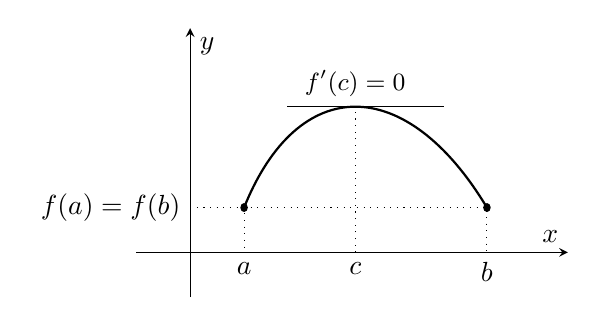
\begin{tikzpicture}
\begin{axis}[
    yscale=0.6,
    axis lines=middle,
    xlabel={$x$},
    ylabel={$y$},
    xtick=\empty,
    ytick=\empty,
    xmin=-1.5, xmax=3.5,
    ymin=-0.5, ymax=2.5,
]
    \node at (0.5,0)  [below] {$a$};
    \node at (2.75,0) [below] {$b$};
    \draw[dotted] (1.53,0) node[below] {$c$} -- 
                  (1.53,1.63) node[above] {\small $f'(c)=0$};
    \draw[thin] (0.9,1.63) -- (2.35,1.63);
    \draw[dotted] (0,0.5) node[left] {$f(a)=f(b)$} -- 
                  (0.5,0.5) -- 
                  (0.5,0);
    \draw[dotted] (0.5,0.5) -- (2.75,0.5) -- (2.75,0);
    \draw[thick] (0.5,0.5) .. controls (1,2) and (2,2) .. 
                 (2.75,0.5);
    \fill (0.5,0.5)  ellipse (0.035 and 0.05);
    \fill (2.75,0.5) ellipse (0.035 and 0.05);
    \draw[very thick,white] (-2,0) -- (-0.5,0);
\end{axis}
\end{tikzpicture}$$
\end{definicion}

\begin{ejemplo}{
    Demuestra que la función:
    \[f(x)=x\ln{(x+2)}\]
    tiene, al menos un punto en el intervalo $(-1,0)$ tal que $f'(x)=0$
}
\end{ejemplo}

\begin{ejemplo}{
    Dada la función:
        \[f(x)=2x+\sen{x}\]
    Demuestra que existe un único punto $c$ tal que $f(c)=2$
}
\end{ejemplo}

\begin{definicion}{Teorema del valor medio de Lagrange.}
Dada una función $f(x)$ continua en el intervalo $[a,b]$ y derivable en el intervalo $(a,b)$, se cumple:
\[\exists c\in(a,b)\mid f'(c)=\frac{f(b)-f(a)}{b-a}\]
$$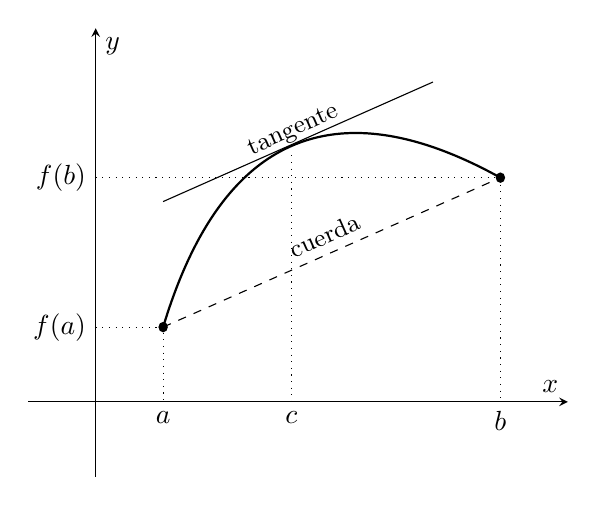
\begin{tikzpicture}
\begin{axis}[
    axis lines=middle,
    xlabel={$x$},
    ylabel={$y$},
    xtick=\empty,
    ytick=\empty,
    xmin=-0.5, xmax=3.5,
    ymin=-0.5, ymax=2.5,
]
    \node at (0.5,0) [below] {$a$};
    \node at (3,0)   [below] {$b$};
    \draw[dotted] (1.45,1.65) -- (1.45,0) node[below] {$c$};
    \draw[dotted] (0,0.5) node[left] {$f(a)$} -- 
                  (0.5,0.5) -- 
                  (0.5,0);
    \draw[dotted] (0,1.5)  node[left] {$f(b)$}-- 
                  (3,1.5) -- 
                  (3,0);
    \draw[thick] (0.5,0.5) .. controls (1,2) and (2,2) .. 
                 (3,1.5);
    \draw[dashed] (0.5,0.5) -- 
                  (3,1.5) node[above,midway,sloped] {\small cuerda};
    \draw (0.5,1.34) -- (2.5,2.14) node[above=-1mm,midway,sloped] {\small tangente};
    \fill (0.5,0.5)  ellipse (0.035 and 0.035);
    \fill (3,1.5) ellipse (0.035 and 0.035);
    %\draw[very thick,white] (-2,0) -- (-0.5,0);
\end{axis}
\end{tikzpicture}$$
\end{definicion}

\begin{ejemplo}{
Dada la función:
    \[f(x)=x^3+2\]
Demuestra que existe algún punto en el intervalo $(-1,1)$, tal que la función $f'(x)=1$. Calcula el valor, o valores en que esto ocurre.
}
\end{ejemplo}

\begin{definicion}{Teorema del valor medio integral.}
Dada una función $f(x)$ continua en el intervalo $[a,b]$, se cumple:
\[\exists c\in(a,b)\,\mid\,f(c)=\dfrac1{b-a}\int_{\,a}^{\,b}\,f(x)\,dx\]
$$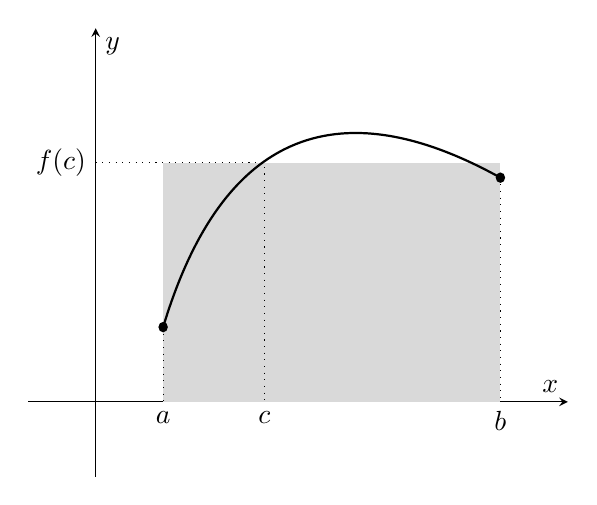
\begin{tikzpicture}
\begin{axis}[
    axis lines=middle,
    xlabel={$x$},
    ylabel={$y$},
    xtick=\empty,
    ytick=\empty,
    xmin=-0.5, xmax=3.5,
    ymin=-0.5, ymax=2.5,
]
    \node at (0.5,0) [below] {$a$};
    \node at (3,0)   [below] {$b$};
    \fill[black!15] (0.5,0) rectangle (3,1.6);
    \draw[dotted] (0,1.6) node[left] {$f(c)$} -- (1.25,1.6) -- (1.25,0) node[below] {$c$};
    \draw[dotted] (0.5,0.5) -- 
                  (0.5,0);
    \draw[dotted] (3,1.5) -- 
                  (3,0);
    \draw[thick] (0.5,0.5) .. controls (1,2) and (2,2) .. 
                 (3,1.5);
    \fill (0.5,0.5)  ellipse (0.035 and 0.035);
    \fill (3,1.5) ellipse (0.035 and 0.035);
    %\draw[very thick,white] (-2,0) -- (-0.5,0);
\end{axis}
\end{tikzpicture}$$
\end{definicion}

\begin{ejemplo}{
Dada la función:
    \[f(x)=x^3+3x+1\]
Encuentra el punto al que se refiere el \emph{Teorema del valor medio integral} en el intervalo $(1,2)$.
}
\end{ejemplo}

\begin{ejemplo}{
Calcula la media aritmética del cuadrado de todos los números reales en el intervalo $[-1,1]$.}
\end{ejemplo}
